\section{The LHCb detector}
\label{sec:Detector}
Located at CERN, the LHC is the largest particle collider in the world and houses a number of experiments. Opposing protons beams are collided at four different
interaction points. At one of these, the LHCb experiment is installed. This detector is constructed as a single-arm forward spectrometer with allows for an optimized detection in the pseudorapidity range
of $2≤\eta≤5$. With the help of this design, the LHCb detector is well suited for the detection of decays that include $b$ and $c$ quarks because the production of these is favored for small angles along the
beam axis. \\
The LHCb experiment consists of serveral sub-detectors, each with a different special purpose. A cross-section of the detector used during the second data-taking run is depicted in \autoref{fig:LHCb_detector}.
\begin{figure}
    \centering
    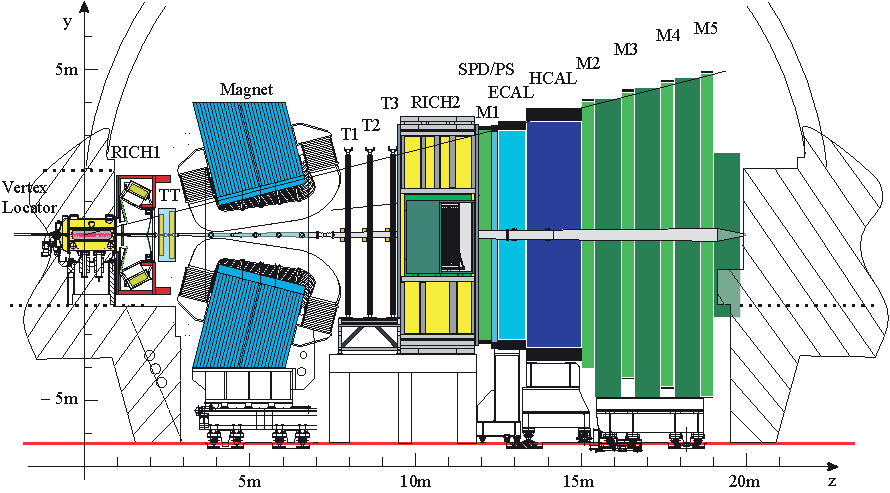
\includegraphics[width=0.8\textwidth]{content/pics/LHCb_detector.pdf}
    \caption{Cross-section of the LHCb detector. A right-handed coordinate system with the z-axis parallel to the beam pipe and the y-axis orientated to the top is used to describe the detector.%
    The different sub-detectors and their purpose and functionality are discussed in this section~\cite{LHCb_detector}.}
    \label{fig:LHCb_detector}
\end{figure}
In the immediate proximity of the interaction point, the Vertex Locator (VELO) is located. Primary and secondary vertices are identified by the 52 silicon pixel modules. The detector is divided into two
halves that are retractable. During the injection phase, the VELO is sitting in its retracted position because the beam is not as focused as during the stable beam phase. Due to the closeness of the VELO to the 
interaction point, the primary veritices can be reconstructed with great accuracy. \\
One of the two Ring Imaging Cherenkov detectors (RICH) is located right before the \qty{1.4}{\tesla} dipole magnet while the other RICH detector is situated behind the tracking stations. Two materials with 
different refractive indices are used in the two RICH detectors to determine the velolcity of the particles via the Cherenkov effect. The implementation of two detectors allows for a larger momentum range 
reconstruction. \\
The position of the particles are detected by the tracking stations, the Tracker Turicensis (TT) and T1-T2. With this information and the previously measured velolcity, the momentum of the particles can
be calculated. \\
For the determination of the energy of the particles, the electromagnetic and hadronic calorimeters (ECAL and HCAL) are employed. To accomplish this task for the ECAL, the shashlik calorimeter 
technology is used. Here, an absorber material and a detector layer of a scintillating material are stacked alternately. The HCAL is constructed similarly but with the scintillating tiles running 
parallel to the beam axis. \\
Muon stations at the end of the detector identify the muons that are passing through the detector. This is accomplished by four multi-wire proportional chambers. \\
Because of the large number of potential events, a trigger system is used to identify interesting decays. The data of these are then saved for further offline analysis.

\section{Analysis strategy}
\label{sec:strategy}
The data used in this analysis consists of three different data samples. One is the actual measured data, which contains reconstructed \printBtoPsiKs \: candidates
and is dominated by combinatorial background and a $B^0_d$ peak. The two other datasets are Monte Carlo simulation samples of the signal decay \printBstoPsiKs \: 
and the control channel decay \printBdtoPsiKs. \\
First, the training samples for the background and the signal need to be defined. In the case for the data of \printBdtoPsiKs \: decay, the background is predominatly combinatorial. The recorded LHCb 
data is used for the training of this classifer. It is to note that the region, where most of the signal is expected, needs to be excluded from this to not get any signal bias into the background classification. \\
The training samples for the signal classification cannot be sourced from the recorded data but must be simulated with Monte Carlo simulations. This leads to the problem of imperfect simulation data 
that does not match the true data of the decay. This is due to not perfect theoretical models and computing constrains. The challenges of this problem can at least be partially overcome by introducing 
computing weights. The here provided simulation data contain a variable called \texttt{kinematic\_weights} that helps to correct for the mismatches between simulation and recorded data. \\
Feature selection is another important aspect of this analysis. The classifier uses a number of features to decide whether the data is background or signal. Features, that can be used here, are extracted
from the control channel \printBtoPsiKs. This decay is similar to the decay \printBstoPsiKs \: and therefore its features can be fed to the classifer.
In priciple, any number of features can be used by a classifier but the runtime scales with the number of features and too many features will eventually lead to overfitting. Some of the here provided features
are also redundant and do not include additional information. \\
For the purpose of ascertaining the best classification threshold, the FOM (\textbf{cite theory???}\eqref{eq:FOM}) is determined by calculating the signal efficiency and number of background events
in the signal region. \\
In the final step, the trained and optimized classifier is used to classify the recorded LHCb data. This leads to the removal of the combinatorial background so that the $B^0$ and $B^0_s$ peaks are clearly
recognizable. The number of signal events can then be extracted. 
